\documentclass[12pt,a4paper]{article}
\usepackage[top=1.5cm, bottom=1.5cm, left=2.0cm, right=1.5cm] {geometry}
\usepackage{amsmath,amssymb,txfonts}
\usepackage{tkz-euclide}
\usepackage{setspace}
\usepackage{lastpage}

\usepackage{tikz,tkz-tab}
%\usepackage[solcolor]{ex_test}
%\usepackage[dethi]{ex_test} % Chỉ hiển thị đề thi
\usepackage[loigiai]{ex_test} % Hiển thị lời giải
%\usepackage[color]{ex_test} % Khoanh các đáp án
\everymath{\displaystyle}

\def\colorEX{\color{purple}}
%\def\colorEX{}%Không tô màu đáp án đúng trong tùy chọn loigiai
\renewtheorem{ex}{\color{violet}Câu}
\renewcommand{\FalseEX}{\stepcounter{dapan}{{\bf \textcolor{blue}{\Alph{dapan}.}}}}
\renewcommand{\TrueEX}{\stepcounter{dapan}{{\bf \textcolor{blue}{\Alph{dapan}.}}}}

%---------- Khai báo viết tắt, in đáp án
\newcommand{\hoac}[1]{ %hệ hoặc
    \left[\begin{aligned}#1\end{aligned}\right.}
\newcommand{\heva}[1]{ %hệ và
    \left\{\begin{aligned}#1\end{aligned}\right.}

%Tiêu đề
\newcommand{\tenso}{}
\newcommand{\tentruong}{}
\newcommand{\tenkythi}{ĐỀ ÔN TẬP}
\newcommand{\tenmonthi}{Môn thi: }
\newcommand{\thoigian}{}
\newcommand{\tieude}[1]{
   \begin{tabular}{cm{3cm}cm{3cm}cm{3cm}}
    {\bf \tenso} & & {\bf \tenkythi} \\
    {\bf \tentruong} & & {\bf \tenmonthi}\\
    && {\bf Thời gian: \bf \thoigian \, phút}\\
    && { \fbox{\bf Mã đề: #1}}
   \end{tabular}\\\\
    
   {Họ tên HS: \dotfill Số báo danh \dotfill}\\
}
\newcommand{\chantrang}[2]{\rfoot{Trang \thepage $-$ Mã đề #2}}
\pagestyle{fancy}
\fancyhf{}
\renewcommand{\headrulewidth}{0pt} 
\renewcommand{\footrulewidth}{0pt}
\usetikzlibrary{shapes.geometric,arrows,calc,intersections,angles,quotes,patterns,snakes,positioning}

\begin{document}
%Thiết lập giãn dọng 1.5cm 
%\setlength{\lineskip}{1.5em}
%Nội dung trắc nghiệm bắt đầu ở đây


\tieude{001}
\chantrang{\pageref{LastPage}}{001}
\setcounter{page}{1}
{\bf PHẦN I. Câu trắc nghiệm nhiều phương án lựa chọn.}
\setcounter{ex}{0}
\Opensolutionfile{ans}[ans/ans001-1]
\begin{ex}
 Cho hàm số $y=f(x)$ liên tục trên $\mathbb{R}$ và có đồ thị $f'(x)$ như hình vẽ. Số điểm cực tiểu của hàm số $y=f(x)$ là 
\begin{center}
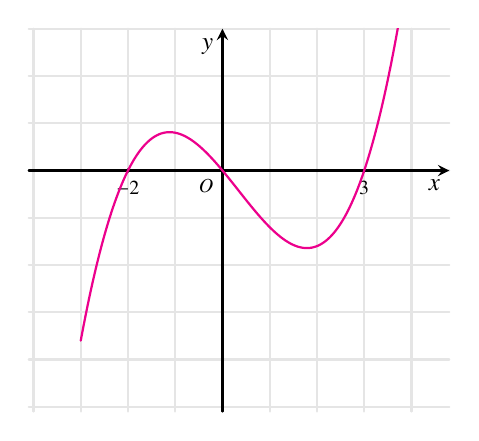
\begin{tikzpicture}[line join=round, line cap=round,>=stealth,thick,scale=0.6]
\tikzset{every node/.style={scale=0.9}}
\draw[gray!20](-4.1,-5.1)grid(4.8,3.00000000000000);
\draw[->] (-4.1,0)--(4.8,0) node[below left] {$x$};
\draw[->] (0,-5.1)--(0,3.00000000000000) node[below left] {$y$};
\draw (0,0) node [below left] {\footnotesize $O$};
\foreach \x in {-2,3}
\draw[thin] (\x,1pt)--(\x,-1pt) node [below] {\footnotesize $\x$};
\foreach \y in {}
\draw[thin] (1pt,\y)--(-1pt,\y) node [left] {\footnotesize $\y$};
\begin{scope}
\clip (-4.1,-5.1) rectangle (4.8,3.00000000000000);
\draw[samples=200,domain=-3:4,smooth,magenta, variable=\x]
plot (\x,{0.2*(\x--2)*(\x-0)*(\x-3)});\end{scope}
\end{tikzpicture}

\end{center}
\choice
{ ${3}$ }
   { \True ${2}$ }
     { ${1}$ }
    { ${0}$ }
\loigiai{ 
 Hàm số đạt cực tiểu tại các điểm $x=-2, x=3$. 
 }\end{ex}

\begin{ex}
 Tìm giá trị lớn nhất của hàm số $y=\ln{\left(x^{2} + 4 x + 7 \right)}$ trên đoạn ${[-3;3]}$.
\\ 
\choice
{ $\ln{39 }$ }
   { $\ln{3 }$ }
     { $\ln{7 }$ }
    { \True $\ln{28 }$ }
\loigiai{ 
 $y'=\frac{2 x + 4}{x^{2} + 4 x + 7}$.

$y'=0 \Rightarrow x=-2$.

$f(-3)=\ln{\left(4 \right)}, f(-2)=\ln{\left(3 \right)}, f(3)=\ln{\left(28 \right)}$.

Vậy giá trị lớn nhất của hàm số $y=\ln{\left(x^{2} + 4 x + 7 \right)}$ trên đoạn ${[-3;3]}$ bằng $\ln{\left(28 \right)}$. 
 }\end{ex}

\begin{ex}
 Cho hình lập phương ${ABCD.A'B'C'D'}$ có độ dài cạnh bằng ${10 a}$. Tính độ dài vectơ $\vec{x}=\overrightarrow{A'B'}+\overrightarrow{A'D'}$ theo ${a}$.\ 
\begin{center}
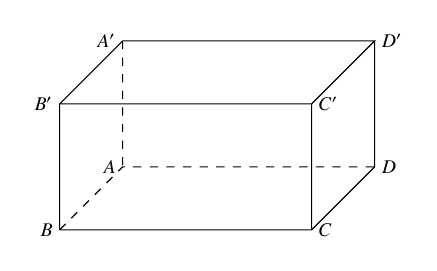
\begin{tikzpicture}[scale=0.8] 
\begin{scriptsize}
\coordinate (A) at (0,0)   node at (A) [left] {$A$};
\coordinate (B) at (-1,-1) node at (B) [left] {$B$};
\coordinate (C) at (3,-1)  node at (C) [right] {$C$};
\coordinate (D) at (4,0)   node at (D) [right] {$D$};
\coordinate (A') at (0,2)   node at (A') [left] {$A'$};
\coordinate (B') at (-1,1) node at (B') [left] {$B'$};
\coordinate (C') at (3,1)  node at (C') [right] {$C'$};
\coordinate (D') at (4,2)   node at (D') [right] {$D'$};
\draw [dashed] (B)--(A)--(D) (A')--(A);
\draw (A')--(B')--(C')--(D')--(A') (B')--(B) (C')--(C) (D')--(D);
\draw (B)--(C)--(D);
\end{scriptsize}
\end{tikzpicture}

\end{center}
\choice
{ ${20 a}$ }
   { ${40 a}$ }
     { \True $10 \sqrt{2} a$ }
    { $10 \sqrt{3} a$ }
\loigiai{ 
 $|\vec{x}|=|\overrightarrow{A'B'}+\overrightarrow{A'D'}|=|\overrightarrow{A'C'}|=10 a.\sqrt 2=10 \sqrt{2} a$. 
 }\end{ex}

\begin{ex}
 Cho hình lập phương ${ABCD.A'B'C'D'}$. Góc giữa hai vectơ $\overrightarrow{A'B'}$ và $\overrightarrow{BC}$ bằng 
\begin{center}
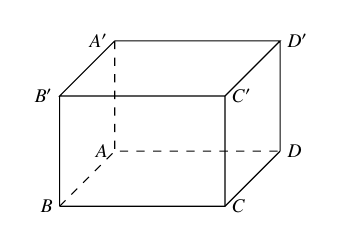
\begin{tikzpicture}[scale=0.7] 
\begin{scriptsize}
\coordinate (A) at (0,0)   node at (A) [left] {$A$};
\coordinate (B) at (-1,-1) node at (B) [left] {$B$};
\coordinate (C) at (2,-1)  node at (C) [right] {$C$};
\coordinate (D) at (3,0)   node at (D) [right] {$D$};
\coordinate (A') at (0,2)   node at (A') [left] {$A'$};
\coordinate (B') at (-1,1) node at (B') [left] {$B'$};
\coordinate (C') at (2,1)  node at (C') [right] {$C'$};
\coordinate (D') at (3,2)   node at (D') [right] {$D'$};
\draw [dashed] (B)--(A)--(D) (A')--(A);
\draw (A')--(B')--(C')--(D')--(A') (B')--(B) (C')--(C) (D')--(D);
\draw (B)--(C)--(D);
\end{scriptsize}
\end{tikzpicture}

\end{center}
\choice
{ \True $90^\circ$ }
   { $60^\circ$ }
     { $120^\circ$ }
    { $45^\circ$ }
\loigiai{ 
 Góc $(\overrightarrow{A'B'}, \overrightarrow{BC})=$ $90^\circ$. 
 }\end{ex}

\begin{ex}
 Cho hai vectơ $\overrightarrow{m}$ và $\overrightarrow{b}$ thỏa mãn $|\overrightarrow{m}|=5,|\overrightarrow{b}|=4$ và $\overrightarrow{m}.\overrightarrow{b}=4$. Tính $|5\overrightarrow{m}-\overrightarrow{b}|$.\ 
\choice
{ \True ${\sqrt{601}}$ }
   { ${\sqrt{661}}$ }
     { ${\sqrt{21}}$ }
    { ${3}$ }
\loigiai{ 
 $|5\overrightarrow{m}-\overrightarrow{b}|^2=(5\overrightarrow{m}-\overrightarrow{b})^2=25\overrightarrow{m}^2-10\overrightarrow{m}\overrightarrow{b}+\overrightarrow{b}$

$=25.5^2-10.4+1.4^2=601$.

Suy ra $|5\overrightarrow{m}-\overrightarrow{b}|=\sqrt{601}$. 
 }\end{ex}

\begin{ex}
 Trong hệ trục tọa độ ${Oxyz}$, cho hai véctơ $\overrightarrow{d}=(7 - m;-6;-1)$ và $\overrightarrow{w}=(5;8 m;-6)$. Tìm các giá trị của ${m}$ để vectơ ${\overrightarrow{d}}$ và vectơ ${\overrightarrow{w}}$ vuông góc.\\ 
\choice
{ $\displaystyle {m=\frac{7}{9}}$ }
   { $\displaystyle {m=\frac{306}{53}}$ }
     { $\displaystyle {m=\frac{29}{9}}$ }
    { \True $\displaystyle {m=\frac{41}{53}}$ }
\loigiai{ 
 $\overrightarrow{d}\bot \overrightarrow{w} \Leftrightarrow \overrightarrow{d}.\overrightarrow{w}=0$$\displaystyle \Leftrightarrow (7 - m).5 + (-6)(8 m) +(-1).(-6)=0\Leftrightarrow m=\frac{41}{53}$. 
 }\end{ex}

\begin{ex}
 Trong hệ trục tọa độ ${Oxyz}$, cho hai véctơ $\overrightarrow{u}(6;-3;-1)$ và $\overrightarrow{c}(4;-6;-5)$. Tọa độ vectơ $4\overrightarrow{u}-6\overrightarrow{c}$ là\\ 
\choice
{ $(-32; 24; 29)$ }
   { \True $(0; 24; 26)$ }
     { $(28; 12; -9)$ }
    { $(10; -9; -6)$ }
\loigiai{ 
 $4\overrightarrow{u}-6\overrightarrow{c}=(0; 24; 26)$. 
 }\end{ex}

\begin{ex}
 Trong không gian với hệ tọa độ ${Oxyz}$, cho các điểm ${A(2;8;-9), B(7;9;-14)}$ và ${C(10;-12;-10)}$ .
Tìm tọa độ điểm ${I}$ sao cho ${ABCI}$ là hình bình hành.\\ 
\choice
{ ${ (19; 5; -33) }$ }
   { ${ (-15; 11; 15) }$ }
     { ${ (-1; 29; -13) }$ }
    { \True ${ (5; -13; -5) }$ }
\loigiai{ 
  ${ABCI}$ là hình bình hành khi ${\overrightarrow{AB}=\overrightarrow{IC}}$.
Suy ra: ${I=(10+2-7; -12+8-9; -10-9+14)=}$ ${ (5; -13; -5) }$. 
 }\end{ex}

\begin{ex}
 Cho mẫu số liệu ghép nhóm về điểm thi và số người dự thi như sau:
 
\begin{center}\begin{tabular}{|c|c|c|c|c|c|c|}
        \hline
        Điểm thi   & [0 ; 3,5) & [3,5 ; 7) & [7 ; 10,5) & [10,5 ; 14) & [14 ; 17,5)\\  
        \hline 
        Số người dự thi & 3 & 19 & 17 & 8 & 6 \\ 
        \hline 
    \end{tabular}
\end{center}
 Khoảng biến thiên của mẫu số liệu ghép nhóm là.
\choice
{ $ {7,0}$ }
   { $ {9}$ }
     { \True ${17,5}$ }
    { $ {8,0}$ }
\loigiai{ 

 Khoảng biến thiên của mẫu số liệu ghép nhóm là: $17,5 - 0,0=17,5$ 
 }\end{ex}

\begin{ex}
 Cho mẫu số liệu ghép nhóm về lương(triệu đồng) và số nhân viên như bảng sau. Tìm khoảng tứ phân vị của mẫu số liệu ghép nhóm đã cho.
 
\begin{center}\begin{tabular}{|c|c|c|c|c|c|c|}
        \hline
        Lương(triệu đồng)   & [7 ; 12) & [12 ; 17) & [17 ; 22) & [22 ; 27) & [27 ; 32) & [32 ; 37)\\  
        \hline 
        Số nhân viên & 5 & 3 & 13 & 9 & 15 & 4 \\ 
        \hline 
    \end{tabular}
\end{center}
\choice
{ \True ${10,62}$ }
   { ${5,31}$ }
     { ${5,31}$ }
    { ${19,63}$ }
\loigiai{ 

 Tổng tần số là: $N=49$.

Tìm tứ phân vị $Q_1$:

Bước 1: Xác định vị trí của $Q_1$: $Q_1$ nằm ở vị trí $\dfrac{49}{4}=12.2$.

Bước 2: Xác định lớp chứa $Q_1$: Tính tần số tích lũy từ lớp đầu tiên đến khi đạt hoặc vượt qua vị trí của $Q_1$ ta được lớp $[17;22)$.

Bước 3: Xác định các thông số của công thức tính $Q_1$.

 Cận dưới của lớp $[17;22)$ chứa $Q_1$: $L=17$

 Tổng tần số của các lớp trước lớp chứa $Q_1$: $F=8$

 Tần số của lớp chứa $Q_1$: $f=13$.

 Độ rộng lớp chứa $Q_1$: $h=22 - 17=5$.

Áp dụng công thức: $Q_1=L+\left(\dfrac{ \dfrac{N}{4}-F }{f}\right).h=17+\left(\dfrac{ \dfrac{49}{4}-8 }{13}\right).5=\frac{969}{52}$.

Tìm tứ phân vị $Q_3$:

Bước 1: Xác định vị trí của $Q_3$: $Q_3$ nằm ở vị trí $\dfrac{3.49}{4}=36.8$.

Bước 2: Xác định lớp chứa $Q_3$: tính tần số tích lũy từ lớp đầu tiên đến khi đạt hoặc vượt qua vị trí của $Q_3$ ta được lớp $[27;32)$.

Bước 3: Xác định các thông số của công thức tính $Q_3$.

 Cận dưới của lớp $[27;32)$ chứa $Q_3$: $L=27$

 Tổng tần số của các lớp trước lớp chứa $Q_3$: $F=30$

 Tần số của lớp chứa $Q_3$: $f=15$.

 Độ rộng lớp chứa $Q_3$: $h=32 - 27=5$.

Áp dụng công thức: $Q_3=L+\left(\dfrac{ \dfrac{3N}{4}-F }{f}\right).h=27+\left(\dfrac{ \dfrac{3.49}{4}-30 }{15}\right).5=\frac{117}{4}$.

Khoảng tứ phân vị là: $\Delta_Q=\frac{117}{4}-\frac{969}{52}=\frac{138}{13}=10,62$. 
 }\end{ex}

\begin{ex}
 Một đường tròn có bán kính bằng ${15}$ cm. Cung trên đường tròn đó có số đo là ${260}^\circ$ thì có độ dài bằng\\ 
\choice
{ $\frac{65 \pi}{9}$ }
   { \True $\frac{65 \pi}{3}$ }
     { $\frac{65 \pi}{6}$ }
    { $\frac{221 \pi}{9}$ }
\loigiai{ 
 Độ dài của cung tròn là: $l=\dfrac{15.260}{180}\pi=\frac{65 \pi}{3}$. 
 }\end{ex}

\begin{ex}
 Tìm các giá trị của tham số $m$ để phương trình $6 \sin{2 x }+3 - m=0$ có nghiệm.
\choice
{ $6 \le m \le 3$ }
   { \True $-3 \le m \le 9$ }
     { $-3 \le m \le 9$ }
    { $3 \le m \le 9$ }
\loigiai{ 
 $6 \sin{2 x }+3 - m=0 \Rightarrow \sin{2 x }=\dfrac{m - 3 }{6}$ có nghiệm khi$-1\le \dfrac{m - 3 }{6} \le 1 $

$\Rightarrow -6 \le m - 3 \le 6\Rightarrow -3 \le m \le 9$. 
 }\end{ex}

\begin{ex}
 Cho $a=\log 2, b=\log 5$. Hãy biểu diễn $\log_{400}{640}$ theo $a$ và $b$.
 
\choice
{ $P={\dfrac{7b}{4a +5}}$ }
   { $P={\dfrac{7b +2}{4a}}$ }
     { $P={\dfrac{b -7}{4a - 4}}$ }
    { \True $P={\dfrac{b + 7a}{4a +2b}}$ }
\loigiai{ 

 $P=\log_{400}{640}=\dfrac{ \log (5.2^{7}) } { \log (2^{4}.5^{2}) }
= \dfrac{\log 5 + \log 2^{7} }{ \log 2^{4}+ \log 5^{2} } =\dfrac{b + 7a}{4a +2b}$. 
 }\end{ex}

\begin{ex}
 Nghiệm của phương trình $\log_5(- 6 x - 1) - \log_5(2 x + 6)=2$ là.
 
\choice
{ ${x=\frac{129}{56}}$ }
   { \True ${x=- \frac{151}{56}}$ }
     { ${x=\frac{73}{56}}$ }
    { ${x=\frac{185}{56}}$ }
\loigiai{ 

 Điều kiện: $- 6 x - 1>0$ và $2 x + 6>0$.

$\log_5(- 6 x - 1) - \log_5(2 x + 6)=2\Leftrightarrow \log_5\dfrac{- 6 x - 1}{2 x + 6}=2\Leftrightarrow \dfrac{- 6 x - 1}{2 x + 6}=5^2$

$\Leftrightarrow - 6 x - 1=25(2 x + 6)\Leftrightarrow x=- \dfrac{151}{56}$.

Kết hợp điều kiện ta được ${x=- \dfrac{151}{56}}$. 
 }\end{ex}

\begin{ex}
 Trong các dãy số $(u_n)$ được cho bởi số hạng tổng quát $u_n$ sau, dãy nào là cấp số cộng 
\choice
{ $u_n=2^n$ }
   { \True $u_n=6 n + 6$ }
     { $u_n=2^{n+1}$ }
    { $u_n=n^{2} - 1$ }
\loigiai{ 
 $u_n=6 n + 6$ là số hạng tổng quát của cấp số cộng vì có  $u_{n+1}-u_n=6$. 
 }\end{ex}

\begin{ex}
 Cho hàm số $f(x)=\left\{ \begin{array}{l} 
  3 x^{2} + x + 3 \text{ khi } x \ge 1  \\ 
 11 - 3 x \text{          khi  } x < 1  
 \end{array} \right.$. Tìm khẳng định đúng.\\ 
\choice
{ Hàm số liên tục tại $x=1$ }
   { Hàm số liên tục tại mọi $x\in \mathbb{R}$ }
     { Hàm số không liên tục tại $x=3$ }
    { \True Hàm số không liên tục tại $x=1$ }
\loigiai{ 
  
 }\end{ex}

\begin{ex}
 Cho hình chóp ${S.ABCD}$ có đáy là hình chữ nhật, $SD\bot (ABCD)$. Biết $DA=2a,DC=5a$. Gọi ${G}$ là điểm thuộc cạnh ${SB}$ sao cho $S{G}=3GB$. Tính khoảng cách từ điểm ${G}$ đến mặt phẳng $(SDA)$.\\ 
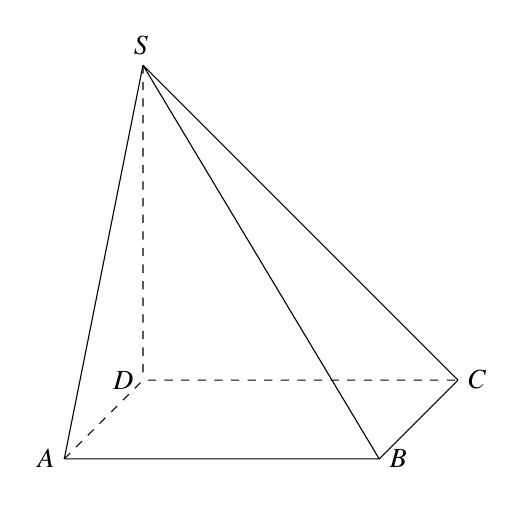
\begin{tikzpicture}
\coordinate (D) at (0,0)   node at (D) [left] {$D$};
\coordinate (A) at (-1,-1) node at (A) [left] {$A$};
\coordinate (B) at (3,-1)  node at (B) [right] {$B$};
\coordinate (C) at (4,0)   node at (C) [right] {$C$};
\coordinate (S) at (0,4)   node at (S) [above] {$S$};
\draw [dashed] (A)--(D)--(C) (S)--(D); 
\draw (A)--(B)--(C) (S)--(A) (S)--(B) (S)--(C); 
\end{tikzpicture}

\choice
{ ${\frac{3}{2}a}$ }
   { \True ${\frac{15}{4}a}$ }
     { ${15a}$ }
    { ${\frac{8}{3}a}$ }
\loigiai{ 
  Vì $BA \bot DA, BA\bot SD \Rightarrow BA \bot (SDA)$. Suy ra $d(B,(SDA))=BA=5a$.

$\dfrac{ d(G,(SDA)) } { d(B,(SDA)) } = \dfrac{SG} {SB} = \frac{3}{4}$$\Rightarrow d(G,(SDA) = \frac{3}{4} d(B,(SDA)) = \frac{3}{4} 5a=\frac{15}{4}a$. 
 }\end{ex}

\begin{ex}
 Một thư viện có ${6}$ cuốn truyện khoa học viễn tưởng và ${10}$ cuốn truyện cổ tích, các cuốn truyện là khác nhau. Chọn ngẫu nhiên ${5}$ cuốn truyện từ thư viện. Tính xác suất của biến cố "Cả ${5}$ cuốn truyện được chọn đều cùng thể loại truyện".
 
\choice
{ ${\dfrac{43}{87360}}$ }
   { ${\dfrac{1}{728}}$ }
     { ${\dfrac{3}{52}}$ }
    { \True ${\dfrac{43}{728}}$ }
\loigiai{ 

 Số cách chọn ${5}$ cuốn truyện là: $C^{5}_{16}=4368$.

Số cách chọn ${5}$ cuốn truyện từ cuốn truyện khoa học viễn tưởng là: $C^{5}_{6}=6$.

Số cách chọn ${5}$ cuốn truyện từ cuốn truyện cổ tích là: $C^{5}_{10}=252$.

Xác suất cần tính là: $P=\dfrac{6+252} {4368}=\dfrac{43}{728}$. 
 }\end{ex}

\begin{ex}
 Từ các chữ  số $\{ {0, 1, 3, 5, 6, 7, 8, 9} \}$ có thể lập được bao nhiêu số tự nhiên gồm 5 chữ số khác nhau?
 
\choice
{ ${56}$ }
   { ${6721}$ }
     { ${6720}$ }
    { \True ${5880}$ }
\loigiai{ 

 Gọi $\overline{a_1a_2a_3a_4a_5}$ là số cần lập.
Chọn $a_1 \ne 0$ có $7$ cách.
Mỗi cách chọn một bộ ${a_2,a_3,a_4,a_5}$ là một chỉnh hợp chập ${4}$ của ${7}$ phần tử.
Số cách lập là: $7.A^{4}_{7} =5880$.
 
 }\end{ex}

\Closesolutionfile{ans}
{\bf PHẦN II. Câu trắc nghiệm đúng sai.}
\setcounter{ex}{0}
\Opensolutionfile{ans}[ans/ans001-2]
\begin{ex}
 Cho bảng số liệu ghép nhóm về điểm thi và số người dự thi như hình dưới đây. Xét tính đúng-sai của các khẳng định sau:
\begin{center}
\begin{tabular}{|c|c|c|c|c|c|c|}
        \hline
        Điểm thi   & [2 ; 4,5) & [4,5 ; 7) & [7 ; 9,5) & [9,5 ; 12) & [12 ; 14,5) & [14,5 ; 17)\\  
        \hline 
        Số người dự thi & 4 & 1 & 11 & 4 & 13 & 2 \\ 
        \hline 
    \end{tabular}

\end{center}
 Xét tính đúng sai của các khẳng định sau.
\choiceTFt
{ \True  Khoảng biến thiên của mẫu số liệu là 15.0 }
   { \True  Tứ phân vị thứ nhất bằng ${7,85}$ }
     { \True  Tứ phân vị thứ ba bằng ${13,20}$ }
    { Khoảng tứ phân vị bằng ${6,35}$ }
\loigiai{ 
 

 a) Khẳng định đã cho là khẳng định đúng.

 Khoảng biến thiên của mẫu số liệu là: $17.0 - 2.0$.

b) Khẳng định đã cho là khẳng định đúng.

 Tìm tứ phân vị $Q_1$:

Tổng tần số là: $N=35$.

Bước 1: Xác định vị trí của $Q_1$: $Q_1$ nằm ở vị trí $\dfrac{35}{4}=8.8$.

Bước 2: Xác định lớp chứa $Q_1$: Tính tần số tích lũy từ lớp đầu tiên đến khi đạt hoặc vượt qua vị trí của $Q_1$ ta được lớp $[7.0;9.5)$.

Bước 3: Xác định các thông số của công thức tính $Q_1$.

 Cận dưới của lớp $[7.0;9.5)$ chứa $Q_1$: $L=7.0$

 Tổng tần số của các lớp trước lớp chứa $Q_1$: $F=5$

 Tần số của lớp chứa $Q_1$: $f=11$.

 Độ rộng lớp chứa $Q_1$: $h=9.5 - 7.0=2.5$.

Áp dụng công thức: $Q_1=L+\left(\dfrac{ \dfrac{N}{4}-F }{f}\right).h=7.0+\left(\dfrac{ \dfrac{35}{4}-5 }{11}\right).2.5=7,85$.



c) Khẳng định đã cho là khẳng định đúng.

 Tìm tứ phân vị $Q_3$:

Tổng tần số là: $N=35$.

Bước 1: Xác định vị trí của $Q_3$: $Q_3$ nằm ở vị trí $\dfrac{3.35}{4}=26.2$.

Bước 2: Xác định lớp chứa $Q_3$: tính tần số tích lũy từ lớp đầu tiên đến khi đạt hoặc vượt qua vị trí của $Q_3$ ta được lớp $[12.0;14.5)$.

Bước 3: Xác định các thông số của công thức tính $Q_3$.

 Cận dưới của lớp $[12.0;14.5)$ chứa $Q_3$: $L=12.0$

 Tổng tần số của các lớp trước lớp chứa $Q_3$: $F=20$

 Tần số của lớp chứa $Q_3$: $f=13$.

 Độ rộng lớp chứa $Q_3$: $h=14.5 - 12.0=2.5$.

Áp dụng công thức: $Q_3=L+\left(\dfrac{ \dfrac{3N}{4}-F }{f}\right).h=12.0+\left(\dfrac{ \dfrac{3.35}{4}-20 }{13}\right).2.5=13,20$.



d) Khẳng định đã cho là khẳng định sai.

  $Q_1=L+\left(\dfrac{ \dfrac{N}{4}-F }{f}\right).h=7.0+\left(\dfrac{ \dfrac{35}{4}-5 }{11}\right).2.5=\frac{691}{88}$.

$Q_3=L+\left(\dfrac{ \dfrac{3N}{4}-F }{f}\right).h=12.0+\left(\dfrac{ \dfrac{3.35}{4}-20 }{13}\right).2.5=\frac{1373}{104}$.

Khoảng tứ phân vị là: $\Delta_Q=\frac{1373}{104}-\frac{691}{88}=\frac{765}{143}=5,3$.



 
 }\end{ex}

\begin{ex}
 Cho hình chóp ${S.ABC}$ có đáy là tam giác đều, $SC\bot (ABC)$. Biết $CA=4a,SC=4 \sqrt{5}a$.

\begin{tikzpicture}
\coordinate (C) at (0,0)   node at (C) [left] {$C$};
\coordinate (A) at (1,-2) node at (A) [left] {$A$};
\coordinate (B) at (4,0)   node at (B) [right] {$B$};
\coordinate (S) at (0,4)   node at (S) [above] {$S$};
\draw [dashed] (C)--(B) ; 
\draw (C)--(A) (A)--(B) (S)--(C) (S)--(A) (S)--(B); 
\end{tikzpicture}

 Xét tính đúng sai của các khẳng định sau
\choiceTF
{ \True Góc giữa đường thẳng ${SA}$ và mặt phẳng ${(ABC)}$ là $\widehat{SAC}$ }
   { Thể tích của khối chóp đã cho bằng $16 \sqrt{15}a^3$ }
     { Góc giữa hai mặt phẳng $(SAB)$ và $(ABC)$ bằng $65,91^\circ$ }
    { \True Khoảng cách từ điểm ${A}$ đến mặt phẳng ${(SCB)}$ bằng $2 \sqrt{3}a$ }
\loigiai{ 
 a) Khẳng định đã cho là đúng.

Góc giữa đường thẳng ${SA}$ và mặt phẳng ${(ABC)}$ là $\widehat{SAC}$.

$\tan \widehat{SAC}=\dfrac{SC}{CA}=\dfrac{4 \sqrt{5}a}{4a}=\sqrt{5}\Rightarrow \widehat{SAC}=65,91^\circ$.

b) Khẳng định đã cho là sai

$V=\dfrac{1}{3}S_{ABC}.SC=\dfrac{1}{3}.\dfrac{16\sqrt{3}}{4}a^2.4 \sqrt{5}a=\frac{16 \sqrt{15}}{3}a^3$

c) Khẳng định đã cho là khẳng định sai.

Gọi M là trung điểm của ${AB}, CM=2 \sqrt{3}a$.

Góc giữa $(SAB)$ và ${(ABC)}$ là $\widehat{SCM}$.

$\tan \widehat{SCM}=\dfrac{SC}{CM}=\dfrac{4 \sqrt{5}a}{2 \sqrt{3}a}=\frac{2 \sqrt{15}}{3}\Rightarrow \widehat{SCM}=68,83^\circ$.

d) Khẳng định đã cho là khẳng định đúng.

Gọi M là trung điểm của ${CB}, AM=2 \sqrt{3}a$.

AM\bot CB,AM\bot SC \Rightarrow AM \bot (SCB)$.

$d(A,(SCB))=AM=2 \sqrt{3}a$.

 
 }\end{ex}

\Closesolutionfile{ans}
{\bf PHẦN III. Câu trắc nghiệm trả lời ngắn.}
\setcounter{ex}{0}
\Opensolutionfile{ans}[ans/ans001-3]
\begin{ex}
 Cho hàm số $f(x)=\dfrac{3 - 5 x}{x-m}$ với ${m}$ là tham số. Tìm số giá trị nguyên của ${m}$ thuộc khoảng $(-80;80)$ để hàm số nghịch biến trên khoảng $(-\infty;-10)$.
\shortans[oly]{${11}$}

\loigiai{ 
 Tập xác định: $D=\mathbb{R}\backslash \{m\}$.

$f'(x)=\dfrac{5 m - 3} {(x-m)^2}$.

Để hàm số nghịch biến trên khoảng $(-\infty;-10)$ thì:

$\left\{ \begin{array}{l}
		5 m - 3<0 \\ 
 		m \notin (-\infty;-10) 
		\end{array} \right. 
 \Leftrightarrow \left\{ \begin{array}{l} 
		m<\frac{3}{5} \\ 
		m \ge -10
		\end{array} \right. 
\Rightarrow -10\le m <\frac{3}{5}$.

Số các số nguyên là: ${11}$. 
 }\end{ex}

\begin{ex}
  Tại một xí nghiệp chuyên sản xuất vật liệu xây dựng, nếu trong một ngày xí nghiệp sản xuất $x (m^3)$ sản phẩm thì phải bỏ ra các khoản chi phí bao gồm: 7 triệu đồng chi phí cố định; 0,6 triệu đồng chi phí cho mỗi mét khối sản phẩm và $0,003x^2$ triệu đồng chi phí bảo dưỡng máy móc. Biết rằng, mỗi ngày xí nghiệp sản xuất được tối đa 65 $m^3$ sản phẩm.  Tìm chi phí trung bình (triệu đồng) trên mỗi mét sản phẩm thấp nhất mà xí nghiệp cần bỏ ra (làm tròn đến hàng phần trăm).
\shortans[oly]{0,89}

\loigiai{ 
  Đáp án:0,89.

 Tổng chi phí (triệu đồng) để xí nghiệp sản xuất $x (m^3)$ sản phẩm trong một ngày là:

$C(x)=7+0,6x+0,003x^2$ với $0\le x \le 65$.

 Chi phí trung bình (triệu đồng) trên mỗi mét khối sản phẩm là:

 $\overline C(x)=\dfrac{C(x)}{x}=\dfrac{7+0,6x+0,003x^2}{x}$ $=\dfrac{7}{x} + 0,6 + 0,003x$.

 $\overline C'(x)=-\dfrac{7}{x^2}+0,003=\dfrac{0,003x^2-7}{x^2}$.

 $\overline C'(x)=0 \Rightarrow x^2=\frac{7000}{3} \Rightarrow x=\sqrt{\frac{7000}{3}}$.

 Bảng biến thiên:

\begin{center}
 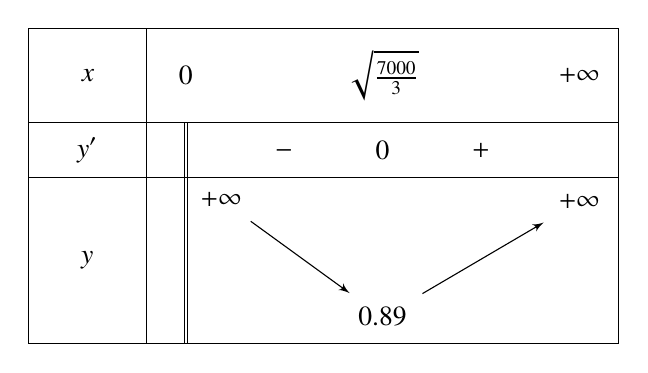
\begin{tikzpicture}
\tkzTabInit[espcl=2.5,lgt=1.5,nocadre=false]
{$x$/1.2,$y'$/0.7,$y$/2.1}
{$0$,$\sqrt{\frac{7000}{3}}$,$+\infty$}
\tkzTabLine{d,-,0,+}
\tkzTabVar{+D+/$ $/$+\infty$,-/$0.89$,+/$+\infty$}
\end{tikzpicture} 
\end{center}
 Từ bảng biến thiên ta thấy chi phí trung bình thấp nhất là:

 $\overline C(\sqrt{\frac{7000}{3}})\approx 0,89 $ đạt được khi $x=\sqrt{\frac{7000}{3}} \approx 48,0$. 
 }\end{ex}

\begin{ex}
 Cho hai vectơ $\overrightarrow{m}$ và $\overrightarrow{n}$ thỏa mãn $|\overrightarrow{m}|=1,|\overrightarrow{n}|=1$ và $\overrightarrow{m}.\overrightarrow{n}=0$. Xét hai vectơ $\overrightarrow{x}=-2\overrightarrow{m}+2\overrightarrow{n}$ và $\overrightarrow{y}=-2\overrightarrow{m}-2\overrightarrow{n}$. Tính $\cos(\overrightarrow{x},\overrightarrow{y})$ (kết quả làm tròn đến hàng phần mười).
\shortans[oly]{0}

\loigiai{ 
 $\overrightarrow{x}.\overrightarrow{y}=(-2\overrightarrow{m}+2\overrightarrow{n}).(-2\overrightarrow{m}-2\overrightarrow{n})=4\overrightarrow{m}^2-4\overrightarrow{n}^2+0\overrightarrow{m}.\overrightarrow{n}=4.1^2-4.1^2+0.(0)=0$.

$|\overrightarrow{x}|=\sqrt{\overrightarrow{x}^2}=\sqrt{(-2\overrightarrow{m}+2\overrightarrow{n})^2}=\sqrt{4\overrightarrow{m}^2+4\overrightarrow{n}^2-8.\overrightarrow{m}.\overrightarrow{n}}=\sqrt{4.1^2+4.1^2-8.(0)}=2 \sqrt{2}$.

$|\overrightarrow{y}|=\sqrt{\overrightarrow{y}^2}=\sqrt{(-2\overrightarrow{m}-2\overrightarrow{n})^2}=\sqrt{4\overrightarrow{m}^2+4\overrightarrow{n}^2+8.\overrightarrow{m}.\overrightarrow{n}}=\sqrt{4.1^2+4.1^2+8.(0)}=2 \sqrt{2}$.

$\cos(\overrightarrow{x},\overrightarrow{y})=\dfrac{\overrightarrow{x}.\overrightarrow{y}}{|\overrightarrow{x}|.|\overrightarrow{y}|}=\dfrac{0}{2 \sqrt{2}.2 \sqrt{2}}\approx 0$

Đáp án: 0 
 }
\end{ex}

\begin{ex}
 Trong không gian ${Oxyz}$, cho điểm $N(\frac{5}{2};-3;-5)$. Biết điểm ${A}$ thuộc trục ${Oy}$ và điểm ${B}$ thuộc mặt phẳng ${(Oxz)}$ sao cho ${N}$ là trung điểm của đoạn thẳng ${AB}$. Gọi ${G(m;n;p)}$ là trung điểm của ${BN}$. Tính $m+n+p$ (kết quả làm tròn đến hàng phần mười).
\shortans[oly]{-5,2}

\loigiai{ 
 Gọi $A(0;a;0), B(b;0;c)$.

Vì ${N}$ là trung điểm của đoạn thẳng ${AB}$ nên$\left\{ \begin{array}{l} 
			\dfrac{b}{2}=\frac{5}{2} \\ 
			\dfrac{a}{2}=-3 \\ 
			\dfrac{c}{2}=-5
			\end{array} \right. \Rightarrow a=-6,b=5,c=-10$.

Suy ra $B(5;0;-10)$.

${G}$ là trung điểm của ${BN} \Rightarrow $$G(\frac{15}{4};- \frac{3}{2};- \frac{15}{2})$.

$m+n+p=\frac{15}{4}- \frac{3}{2}- \frac{15}{2}=- \frac{21}{4}$.

 
 }\end{ex}

\begin{ex}
 Cho mẫu số liệu ghép nhóm về cân nặng(kg) và số người như sau:
\begin{center}
\begin{tabular}{|c|c|c|c|c|c|c|}
        \hline
        Cân nặng(kg)   & [35 ; 41) & [41 ; 47) & [47 ; 53) & [53 ; 59) & [59 ; 65) & [65 ; 71)\\  
        \hline 
        Số người & 24 & 32 & 5 & 4 & 33 & 15 \\ 
        \hline 
    \end{tabular}

\end{center}
 Tính phương sai của mẫu số liệu ghép nhóm trên (kết quả làm tròn đến hàng phần mười).
\shortans[oly]{123,7}

\loigiai{ 
 Các giá trị đại diện của mẫu số liệu là: 38; 44; 50; 56; 62; 68

Tổng tần số là: $n=113$

Số trung bình của mẫu số liệu ghép nhóm là:

$\overline{x}=\dfrac{38.24+44.32+50.5+56.4+62.33+68.15}{ 113}=51,86$.

Phương sai của mẫu số liệu ghép nhóm là:

$S^2=\dfrac{1}{113}(38.24^2+44.32^2+50.5^2+56.4^2+62.33^2+68.15^2)-51,86^2=123,7$.

Đáp án: 123,7 
 }\end{ex}

\Closesolutionfile{ans}

 \begin{center}
-----HẾT-----
\end{center}

 %\newpage 
%\begin{center}
%{\bf BẢNG ĐÁP ÁN MÃ ĐỀ 1 }
%\end{center}
%{\bf Phần 1 }
% \inputansbox{6}{ans001-1}
%{\bf Phần 2 }
% \inputansbox{2}{ans001-2}
%{\bf Phần 3 }
% \inputansbox{6}{ans001-3}
\newpage 



\end{document}